\documentclass[10pt]{beamer}

%\usetheme[progressbar=frametitle]{metropolis}
\usepackage{appendixnumberbeamer}

\usepackage{booktabs}
\usepackage[scale=2]{ccicons}

\usepackage{xspace}
%\newcommand{\themename}{\textbf{\textsc{metropolis}}\xspace}
%%%%%%%%%%%%%%%%%%%%%%%%
\usepackage{minted}

\graphicspath{images/}

%%%%%%%%%%%%%%%%%%%%%%%%
\title{datetime}
\subtitle{A Tale of Pythonic Woe}
% \date{\today}
\date{23 August 2017}
\author{Dave Voutila}
\institute{Sisu Integrated Services, LLC}
% \titlegraphic{\hfill\includegraphics[height=1.5cm]{logo.pdf}}

\begin{document}

\maketitle

\begin{frame}{Table of contents}
  \setbeamertemplate{section in toc}[sections numbered]
  \tableofcontents[hideallsubsections]
\end{frame}

\section{Introduction}
\begin{frame}[fragile]{Backstory}
\begin{itemize}
\item Contributor to \textbf{Flask-Ask}, a Python Amazon Alexa framework.
\item Jumped on \textit{Issue 152: Flask Ask doesn't parse time stamp from Alexa properly...}
\item Things when downhill from there...
\end{itemize}

\end{frame}

\begin{frame}{The Problem}
\begin{center}
	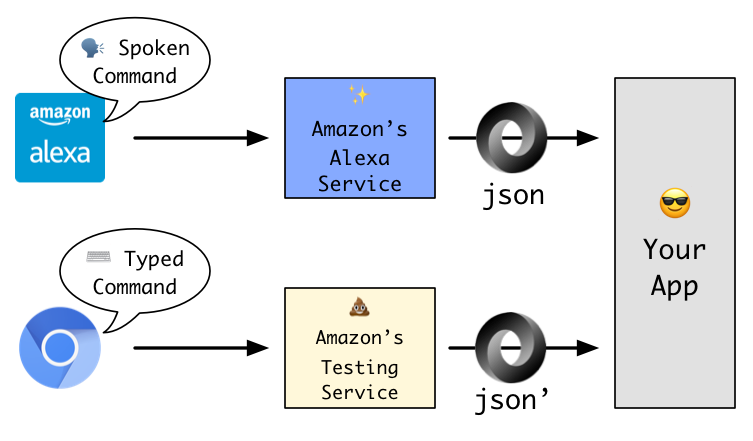
\includegraphics[width=9cm]{./images/alexa-flow.png}
	\begin{alertblock}{Attention}
		json != json'
	\end{alertblock}
\end{center}
\end{frame}

\begin{frame}{A Tale of Two Timestamps}
TODO: Talk about the two timestamps
\end{frame}

\section{Python's datetime}
\begin{frame}{Python and Time ⏱}
\end{frame}
\end{document}

